\chapter{Materiales y métodos} 

% ------------------------------------------------------------------------------------------------------------
% ------------------------------------------------------------------------------------------------------------

\section{Conjunto de datos disponibles}

% ------------------------------------------------------------------------------------------------------------

%\subsection{Radiografías panorámicas maxilofaciales}

Disponemos de un conjunto de datos compuesto por radiografías panorámicas maxilofaciales de individuos de 
diversos países y continentes (véase en la tabla \ref{tab:instituciones_fuente_dataset}), obtenidas con
distintos modelos de máquinas de rayos X
\footnote{
    Los modelos empleados fueron: \textit{Planmeca Promax Digital Panoramic}; \textit{Sirona ORTHOPHOS-XG}, 
    \textit{ORTHOPHOS-DS}, y \textit{SIDEXIS}. Las constantes radiológicas usadas fueron de 66 a a 70 kV, 7 a 
    11 mA, y 15 s.
}. 
Este conjunto de datos ha sido sido proporcionados por Panacea Cooperative Research, empresa \textit{spin-off} 
de la Universidad de Granada.  

\begin{table}[h]
\begin{tabular}{@{}clc@{}}
\toprule
País                                                            & Instituciones                                                                                                                                                            & Nº de ejemplos \\ \midrule
\begin{tabular}[c]{@{}c@{}}Bosnia y \\ Herzegovina\end{tabular} & Universidad de Sarajevo                                                                                                                                                  & 882            \\ \hline
Botsuana                                                        & \begin{tabular}[c]{@{}l@{}}Dos clínicas dentales privadas en \\ Garobone\end{tabular}                                                                                    & 1242           \\ \hline
Chile                                                           & \begin{tabular}[c]{@{}l@{}}Dos clínicas dentales privadas en \\ Santiago y Rancagua\end{tabular}                                                                         & 1016           \\ \hline
\begin{tabular}[c]{@{}c@{}}República \\ Dominicana\end{tabular} & \begin{tabular}[c]{@{}l@{}}Tres clínicas dentales privadas en \\ Santo Domingo, La Vega y Santiago\end{tabular}                                                          & 541            \\ \hline
Japón                                                           & \begin{tabular}[c]{@{}l@{}}Department of Forensic Sciences, \\ Iwate Medical University, Iwate\end{tabular}                                                              & 1045           \\ \hline
Corea                                                           & Catholic University of Korea, Seoul                                                                                                                                      & 500            \\ \hline
Malasia                                                         & \begin{tabular}[c]{@{}l@{}}Faculty of Dentistry Universiti Teknologi \\ MARA Selangor Branch, Selangor\end{tabular}                                                      & 667            \\ \hline
Turquía                                                         & \begin{tabular}[c]{@{}l@{}}Department of Dentomaxillofacial \\ Radiology, Baskent University, Turkey\end{tabular}                                                        & 2323           \\ \hline
Uganda                                                          & \begin{tabular}[c]{@{}l@{}}Department of Dental Morphology with \\ the Université Claude Bernard Lyon 1, \\Faculté d’odontologie, Lyon\end{tabular}                      & 283            \\ \hline
Italia                                                          & \begin{tabular}[c]{@{}l@{}}Department of Surgical Sciences, \\ University of Cagliari\end{tabular}                                                                       & 173            \\ \hline
Kosovo                                                          & \begin{tabular}[c]{@{}l@{}}University Dentistry Clinical Center, \\ Pristina\end{tabular}                                                                                & 1397           \\ \hline
Líbano                                                          & Clínica dental privada en Beirut                                                                                                                                         & 690            \\ \bottomrule
\end{tabular}
\caption[
    Instituciones participantes en la recolección de datos e imágenes
]{   
    Lista de instituciones participantes en la recolección de los datos e imágenes dentales utilizados en el 
    trabajo.
}
\label{tab:instituciones_fuente_dataset}
\end{table}

Este \textit{dataset} incluye:

\begin{itemize}

    \item datos tabulares (en formato CSV), donde cada fila representa un ejemplo (un individuo), con los 
    siguientes campos: un identificador único, sexo del individuo, edad del individuo y ``sample'' 
    (clasificación según el origen geográfico de la radiografía), e

    \item imágenes bidimensionales de radiografías panorámicas maxilofaciales, con una imagen asociada 
    a cada individuo y se identifica mediante su ID único. 

\end{itemize}

Se proporcionan los datos ya preprocesados, por lo que no es necesario realizar tareas adicionales de limpieza 
o transformación previa antes de su análisis.

Se ha ignorado el campo de ``sample'', dado que se trata de una asignación
sesgada y no representa necesariamente una clasificación fiable del origen poblacional de los individuos.
Por tanto, este campo no se emplea en el análisis ni en el entrenamiento de los modelos, centrándose 
exclusivamente en las variables de edad, sexo e imagen.

En el \textit{dataset} hay un total de 10.739 ejemplos, de los que 5.756 son de individuos de sexo femenino 
y 4.983 de sexo masculino. 
Las edades mínima y máxima son 14 y 26 años, respectivamente, y la media son 19,13 años.
En la Figura \ref{fig:histogram_ages} se observa que el número de ejemplos por edad se mantiene relativamente 
constante desde los 14 hasta los 21 años, a partir de los cuales disminuye progresivamente, con una 
representación notablemente menor en los grupos de 24, 25 y 26 años.
 
\begin{figure}[h]
    \centering
    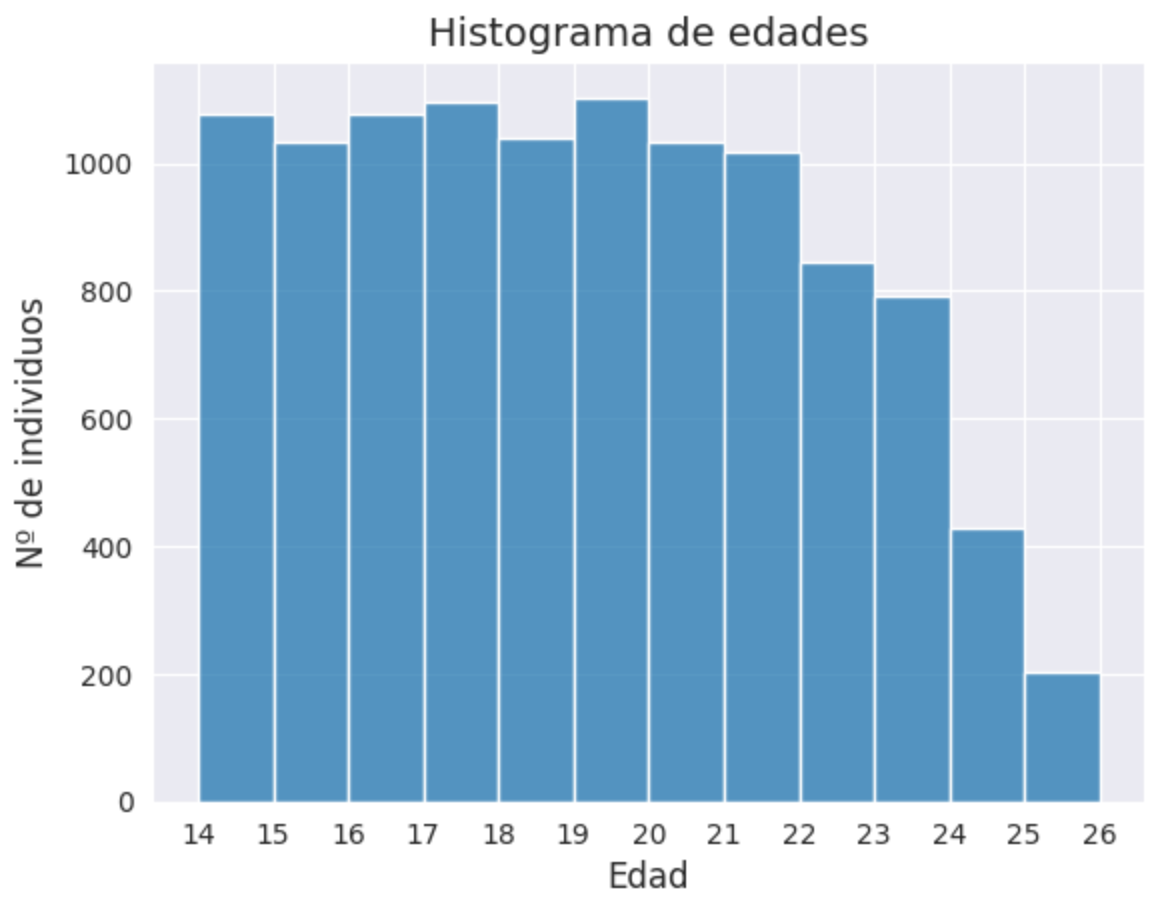
\includegraphics[width=0.7\textwidth]{capitulos/cap_04/imagenes/histogram_ages.png}
    \caption[
        Histograma de edad de los individuos del conjunto de datos disponible.
    ]{
        Histograma de edad de los individuos del conjunto de datos disponible. 
        Elaboración propia.
    } 
    \label{fig:histogram_ages}
\end{figure}

En la Figura \ref{fig:kde_and_boxplot_ages_sex} podemos comprobar cómo en términos relativos la distribución 
de edad por sexo es muy similar, compartiendo ambas prácticamente el mismo rango de edades y patrones de 
dispersión, sin observarse diferencias sustanciales en la mediana ni en la forma general de las 
distribuciones.

\begin{figure}[h]
    \centering
    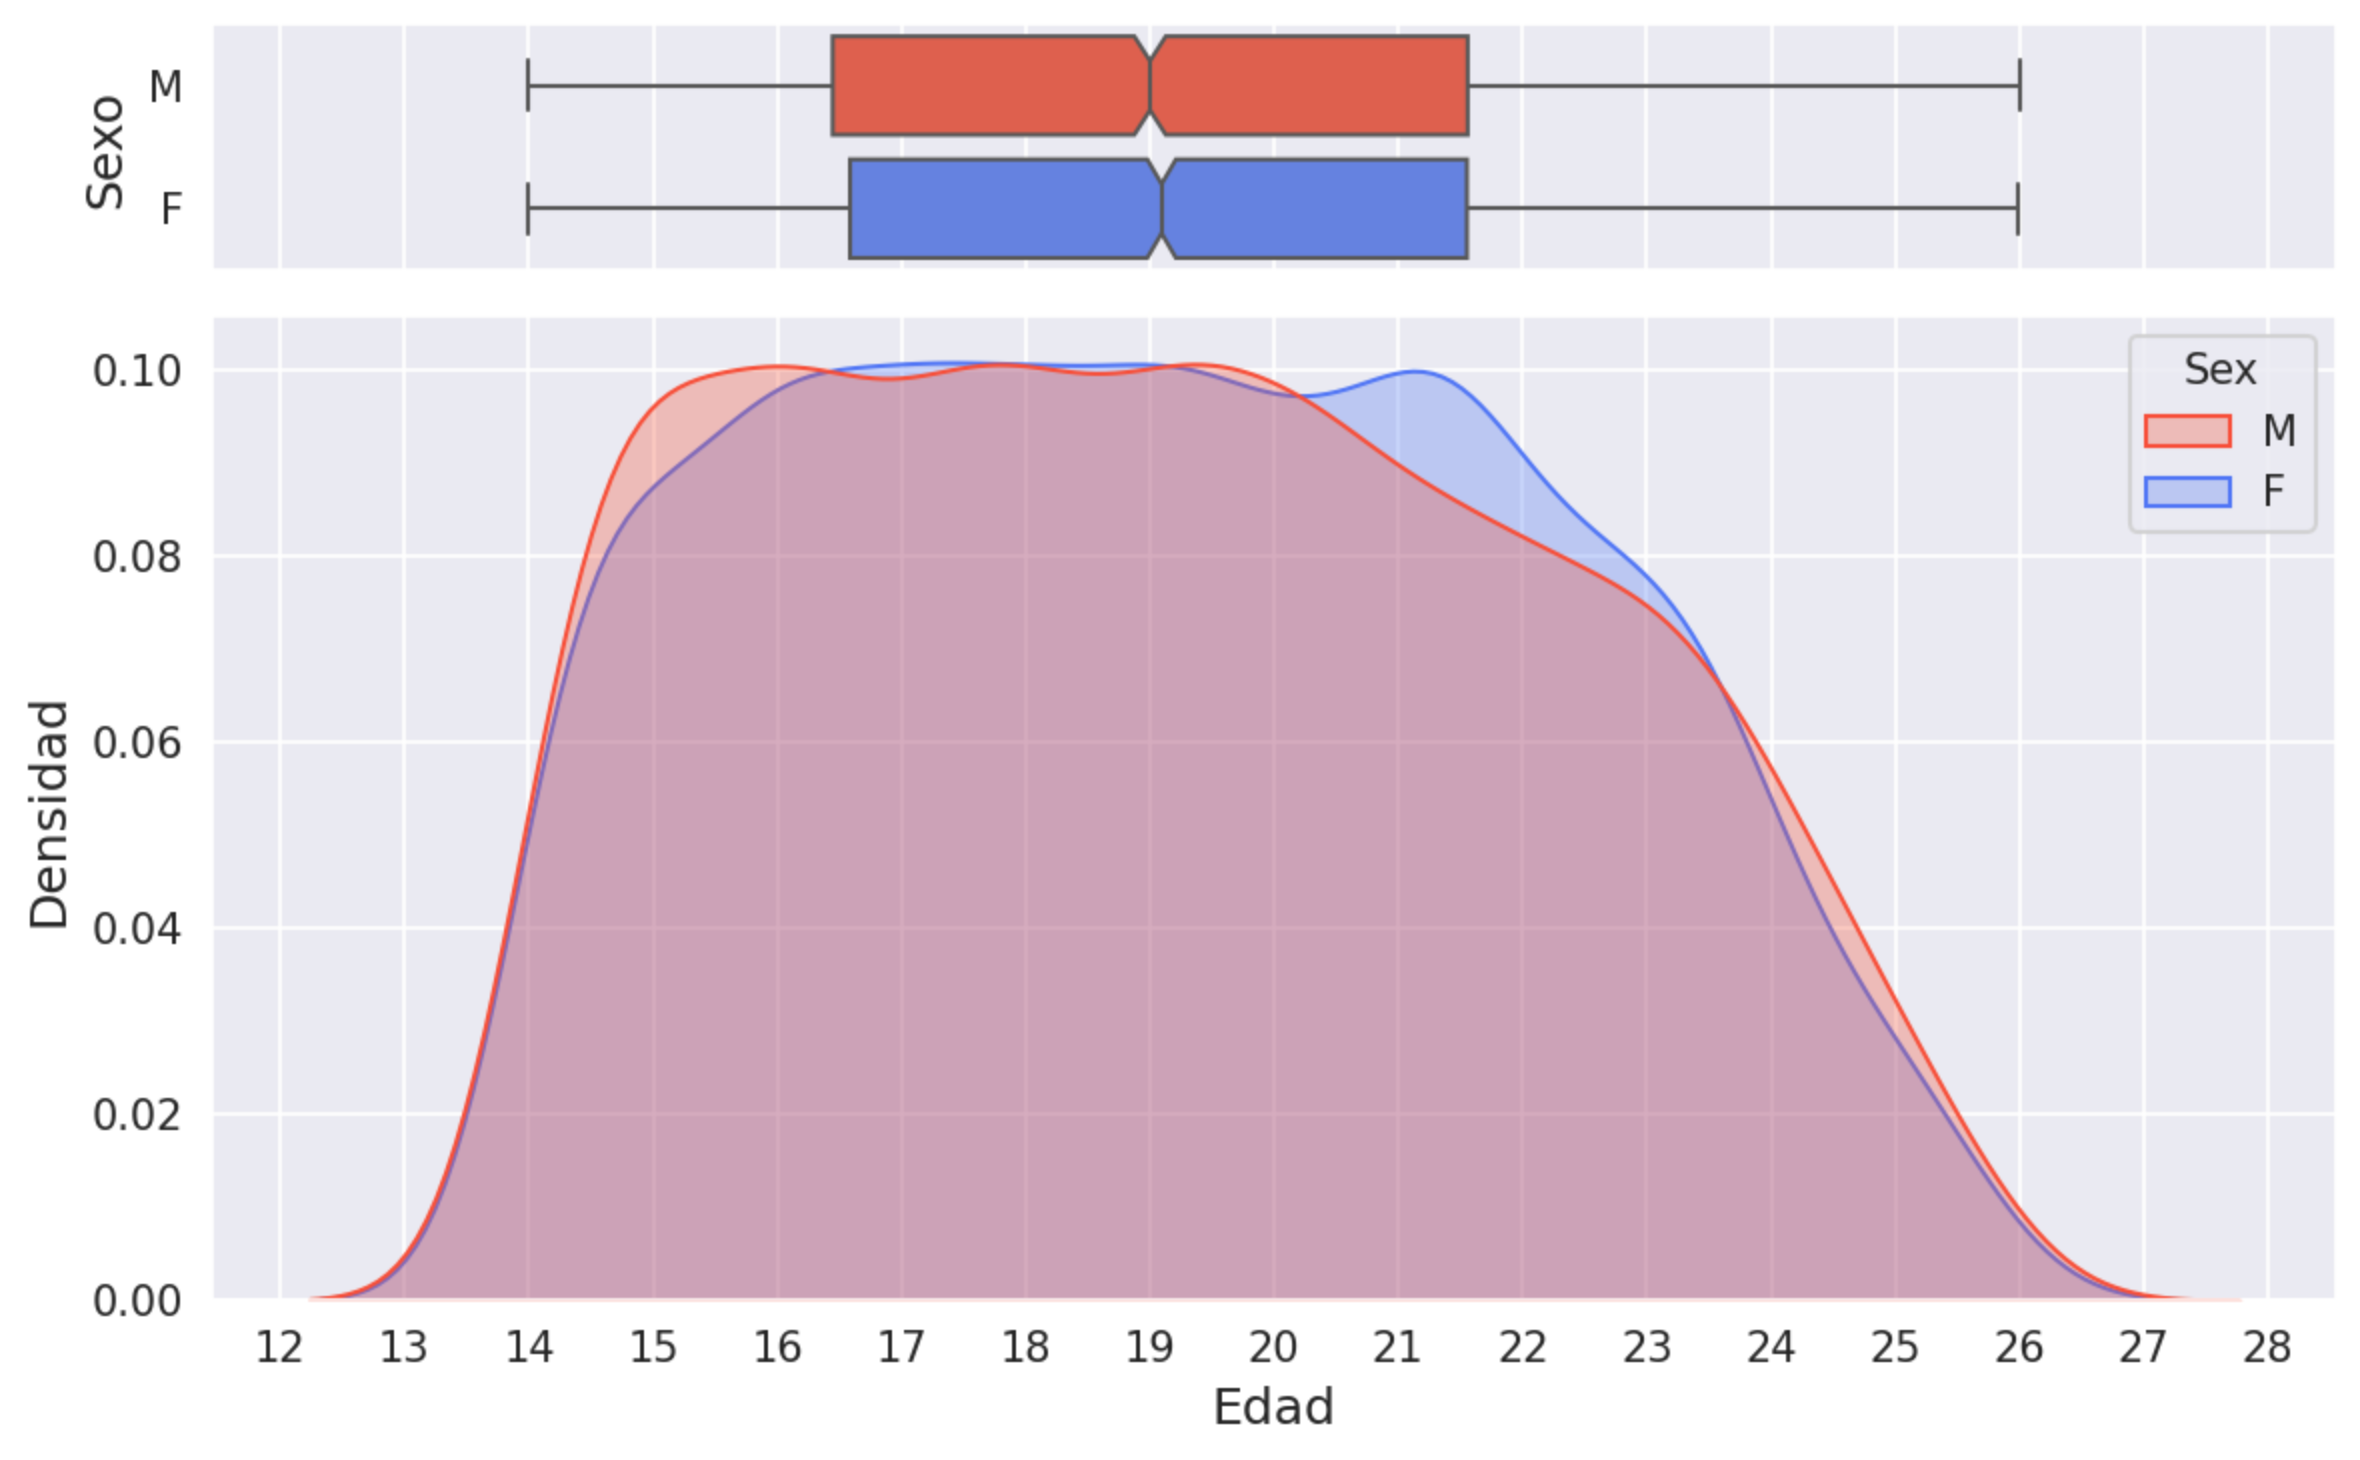
\includegraphics[width=\textwidth]{capitulos/cap_04/imagenes/kdeplot_ages.png}
    \caption[
        Gráficas de densidad y de caja de edad por sexo de los individuos del conjunto de datos disponible.
    ]{
        Gráficas de densidad y de caja de edad por sexo de los individuos del conjunto de datos disponible. 
        Elaboración propia.
    } 
    \label{fig:kde_and_boxplot_ages_sex}
\end{figure}

En conclusión, el dataset presenta en general un buen balance entre clases y edades, lo que permite un 
análisis representativo de la población incluida. No obstante, será necesario examinar con mayor detalle la 
infrarepresentación de los grupos de mayor edad, especialmente a partir de los 22 años, para evaluar su 
posible impacto en el rendimiento y generalización de los modelos entrenados.

Se proporcionan los datos ya divididos en \textit{train} ---con un 80\% de los individuos--- y \textit{test}
---con el 20\% restante---, con la intención de que puedan ser utilizados para entrenar y evaluar modelos de 
predicción. En la Figura \ref{fig:kde_ages_train_test} se puede observar cómo existe una distribución 
edad-sexo similar en los datos de ambos subconjuntos, por lo que se puede asumir que la partición respeta la 
representatividad de la población original, favoreciendo una evaluación más realista del rendimiento de los 
modelos en datos no vistos.

\begin{figure}[h]
        \centering

        \begin{subfigure}[b]{0.47\textwidth}
            \centering
            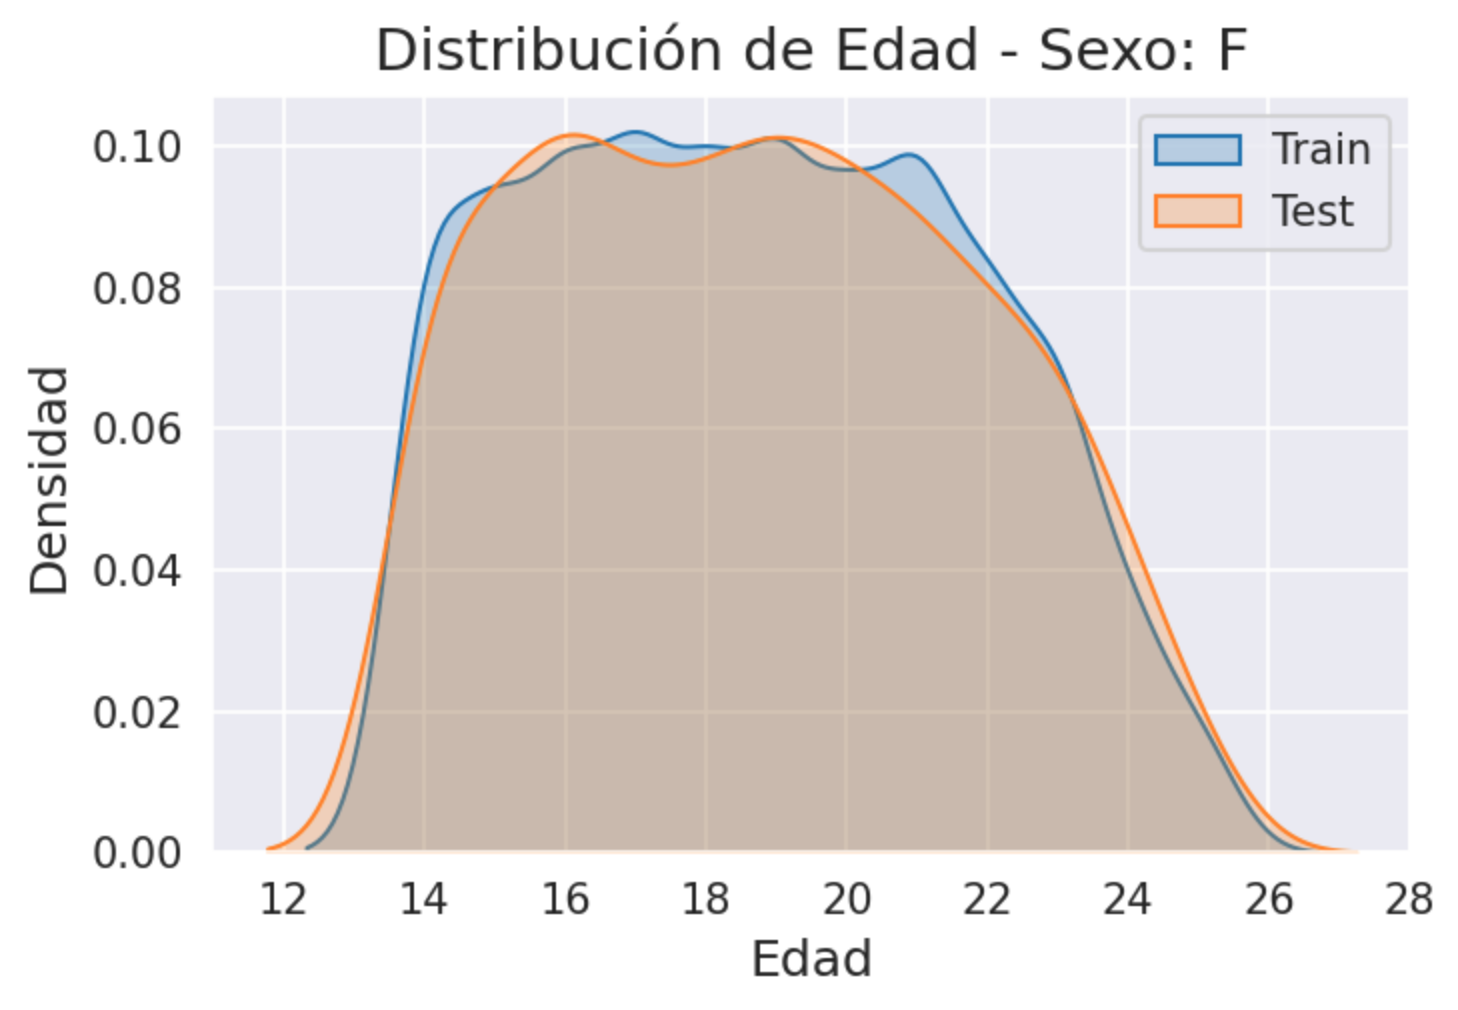
\includegraphics[width=\textwidth]{capitulos/cap_04/imagenes/kde_ages_F.png}
            \caption{Distribución de edad de individuos de sexo femenino.}
            \label{fig:kde_ages_F}
        \end{subfigure}
        \hfill
        \begin{subfigure}[b]{0.47\textwidth}
            \centering
            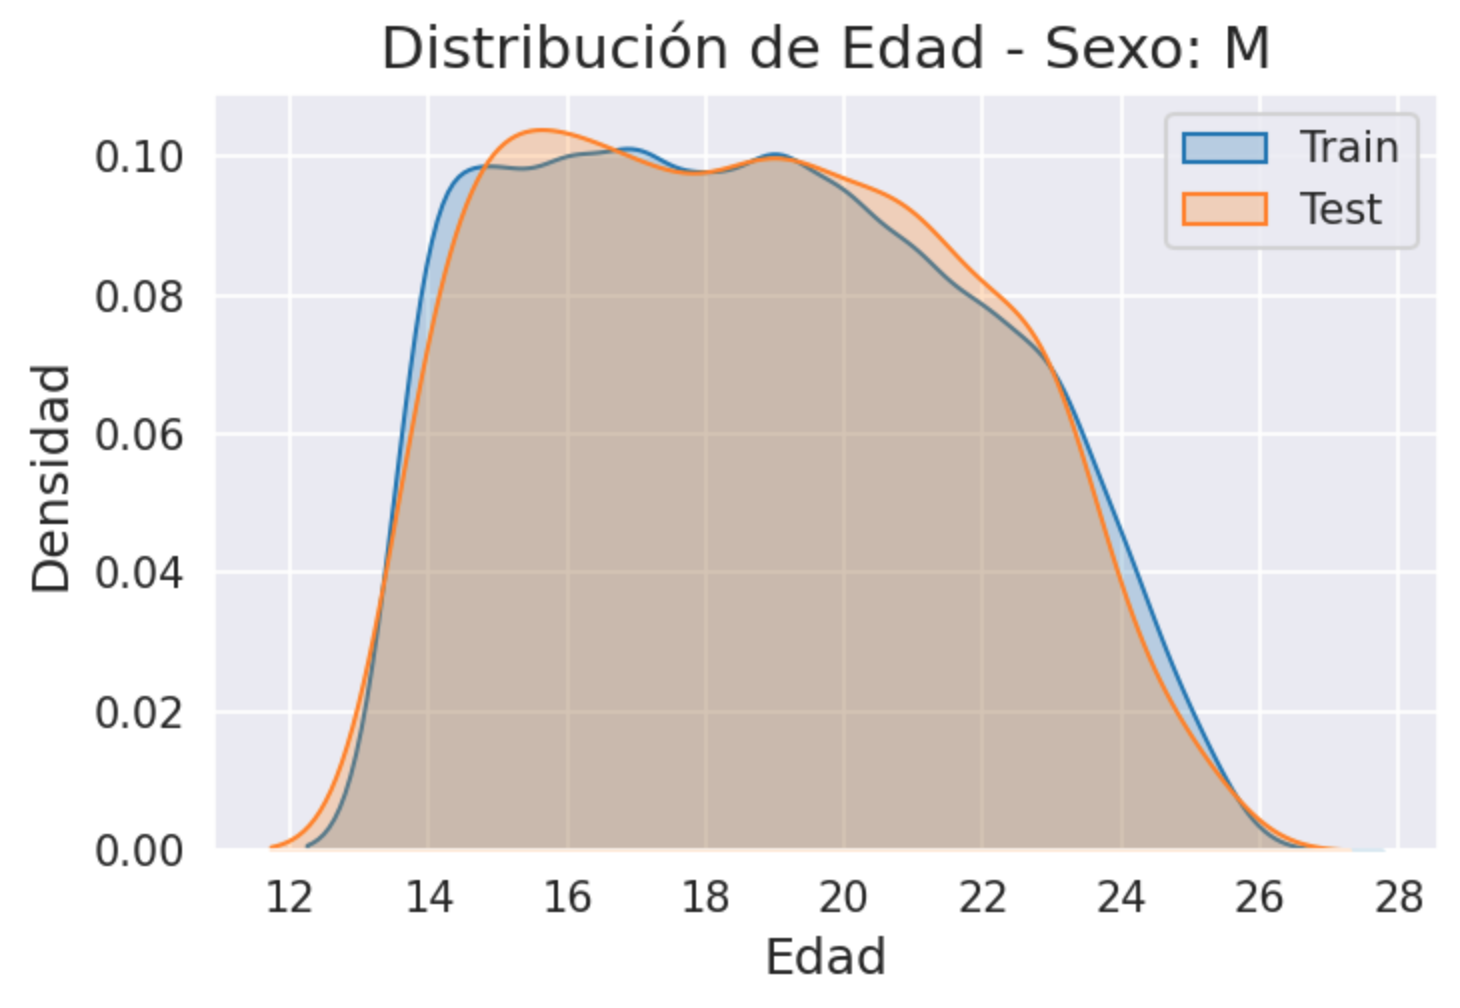
\includegraphics[width=\textwidth]{capitulos/cap_04/imagenes/kde_ages_M.png}
            \caption{Distribución de edad de individuos de sexo masculino.}
            \label{fig:kde_ages_M}
        \end{subfigure}

        \caption[
            Distribución de edad de los individuos del conjunto de datos disponible por sexo.
        ]{
            Distribución de edad de los individuos del conjunto de datos disponible por sexo. 
            Elaboración propia.
        }
        \label{fig:kde_ages_train_test}
    \end{figure}


% ------------------------------------------------------------------------------------------------------------
% ------------------------------------------------------------------------------------------------------------

\section{Problemas planteados}

Como se ha anticipado anteriormente, este trabajo se centrar en los problemas de estimación de edad y ...

% ------------------------------------------------------------------------------------------------------------

\subsection{Problema de estimación de edad}

El problema de \textbf{estimación de edad (\textit{age estimation}, AE)} consiste en predecir la edad 

Este se trata de un problema de regresión, 


% ------------------------------------------------------------------------------------------------------------

\subsection{Estimación de minoría/mayoría de edad}

El problema inmediatamente derivado del anterior es la 
\textbf{estimación de minoría/mayoría de edad (\textit{assessment of the age of majority}, AAM)}.
Este se trata de un problema de clasificación binaria, ...


% ------------------------------------------------------------------------------------------------------------
% ------------------------------------------------------------------------------------------------------------

\section{Métodos propuestos}

\subsection{Arquitectura empleada}

El primer problema propuesto es el de estimación de edad. Partiremos de un planteamiento muy simple: imágenes 
bidimensionales de las radiografías panóramicas maxilofaciales como entrada, y estimación de edad a la salida.
No incorporaremos el sexo del individuo en esta primera aproximación, si bien se explorará en el Anexo X. 
\todo{¿Finalmente incluimos o no el sexo el sexo del individuo?}

Como modelo, empleamos una CNN, dado su buen desempeño en tareas de visión por computador. Específicamente,
implementamos la arquitectura ResNeXt50 \cite{xie2017}, utilizando un modelo entrenado con el \textit{dataset} 
ImageNet
\todo{¿Debería entrar en detalle de por qué ResNeXt50? ¿Comparar sus capacidades con otras arquitecturas CNN?}
\footnote{
    El dataset Imagenet contiene 1.000 clases de objetos. Estas clases abarcan una
    amplia variedad de categorías, como animales (\textit{tiger}, \textit{koala}, \textit{zebra}, ...), 
    vehículos (\textit{ambulance}, \textit{airliner}, \textit{mountain bike}, ...), alimentos 
    (\textit{strawberry}, \textit{pizza}, \textit{bagel}, ...), entre otras. 
}
\cite{deng2009} como punto de partida. Este modelo preentrenado es accesible a través de Pytorch. 

Aunque ResNeXt50 fuera diseñado originalmente para un problema de clasificación de imágenes y entrenado con
un dominio distinto al de nuestro problema, su adaptación a una tarea de estimación de edad es sencilla: 
reemplazar su cabecera de clasificación por una de regresión. Además, el uso de peso preentrenados proporciona
una inicialización más robusta que el entrenamiento desde cero, ya que el modelo ya ha aprendido filtros 
genéricos para detectar características visuales básicas, como bordes o texturas.

% ------------------------------------------------------------------------------------------------------------

\subsection{Regresión cuantílica}

La \textbf{regresión cuantílica (\textit{quantile regression}, QR)} es un tipo de regresión que, a diferencia
de la regresión puntual, predice intervalos o cuantiles específicos de la distribución de la variable 
respuesta, en lugar de solo su media. 
Esta técnica permite modelar límites inferiores y superiores (por ejemplo, el percentil 10\% y 90\%) para
capturar la incertidumbre o heterocedasticidad en los datos.

Esta técnica de regresión puede implementarse en diversos modelos, aunque su implementación difiere 
significativamente. 

En redes neuronales, esta regresión requiere de:

\begin{itemize}

    \item Definir una capa de salida con múltiples neuronas, una por cada cuantil deseado. Por ejemplo, para 
    obtener una región del 90\% con predicción puntual, tendríamos los cuantiles 0.05 y 0.95 para los límites
    inferior y superior, respectivamente, y 0.5 para la predicción puntual. 

    \item Cambiar la función de pérdida por una que admite varias salidas. En general, se suele utilizar la 
    la pérdida \textit{pinball} \cite{steinwart2011}.

    La \textbf{función de pérdida \textit{pinball}} es una generalización de la función de pérdida del MAE,
    que penaliza las predicciones de manera asimétrica según el cuantil objetivo. Para un cuantil 
    $\tau \in \left( 0,1\right)$, se define como:

    $$
    L_\tau(y,\hat{y}) = \left\{
        \begin{array}{rcl}
            \tau \cdot (y-\hat{y}) & \mbox{si} & y \ge \hat{y}
            \\
            (1-\tau) \cdot (\hat{y}-y) & \mbox{si} & y < \hat{y}
        \end{array}
    \right.
    $$

    En la Figura \ref{fig:pinball_loss} podemos apreciar la penalización asimétrica para errores positivos y 
    negativos. 

    \begin{figure}[h]
        \centering
        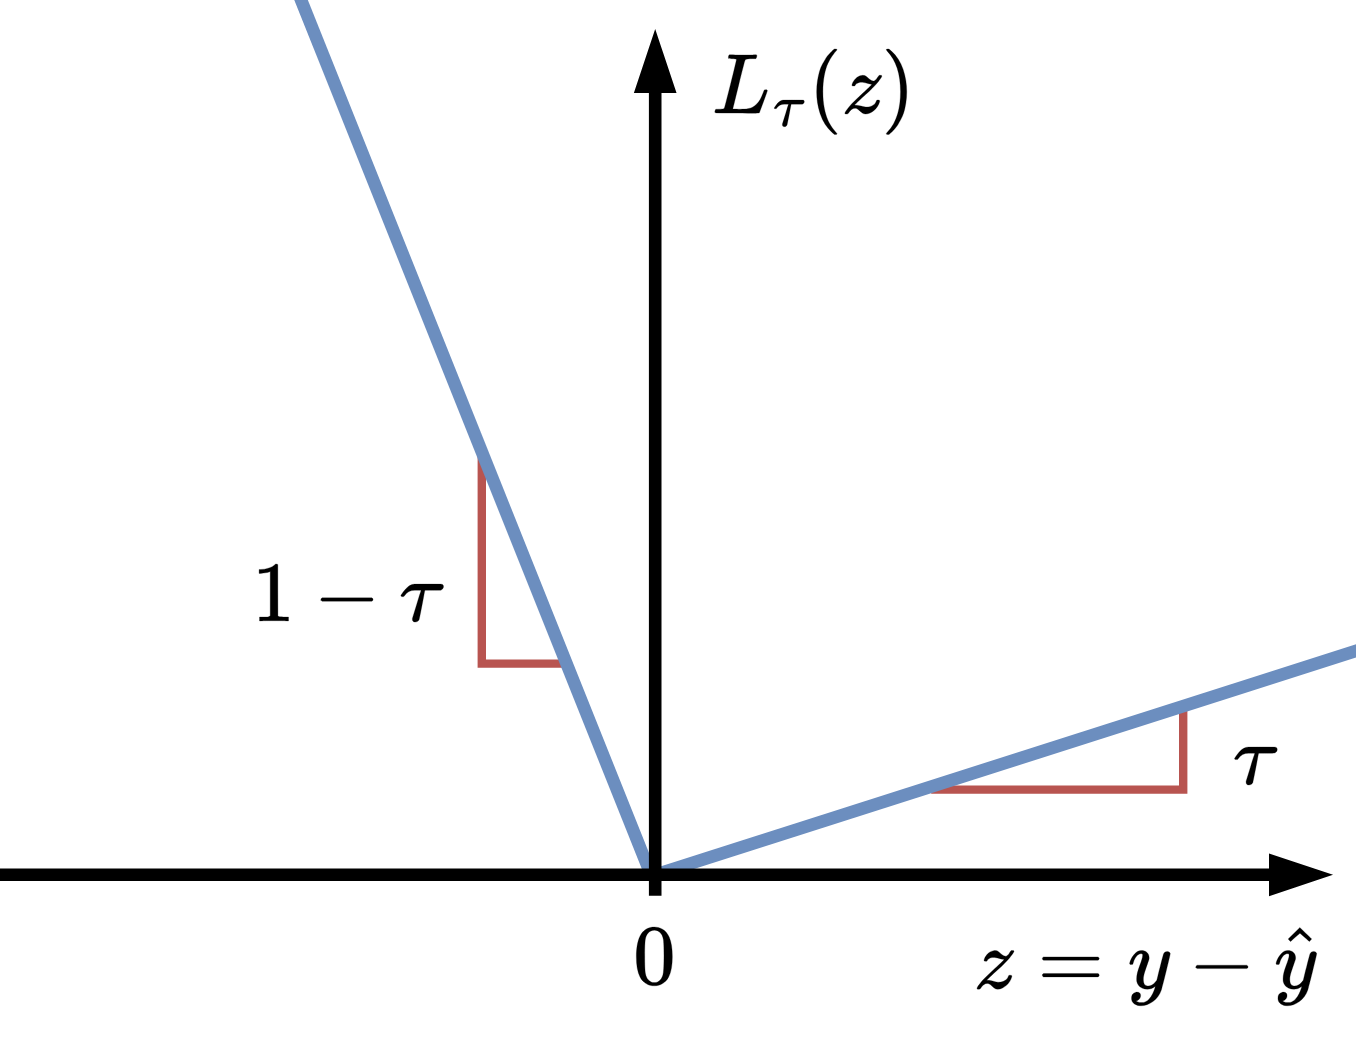
\includegraphics[width=0.5\textwidth]{capitulos/cap_04/imagenes/pinball_loss.png}
        \caption[
            Visualización de la función de pérdida \textit{pinball} para cada valor de error.
        ]{
            Visualización de la función de pérdida \textit{pinball} para cada valor de error.
            Adaptado de la Figura 1 de \cite{romano2019}.
            Esta concretamente muestra la función de pérdida para un cuantil cercano a cero, 
            ya que es más permisivo con los errores positivos que con los negativos.
        } 
        \label{fig:pinball_loss}
    \end{figure}

    Esta función de pérdida, aplicada a múltiples salidas (cada una asociada a un cuantil específico), busca 
    que las predicciones del modelo cubran la proporción deseada de los datos dentro del intervalo definido 
    por los cuantiles. Por ejemplo:

    \begin{itemize}

        \item Para $\tau = 0.05$ y $\tau = 0.95$, el modelo intentará que el 90\% de las observaciones reales 
        ($y$) caigan entre los límites predichos ($\hat{y}{0.05}$ y $\hat{y}{0.95}$).

        \item La mediana ($\tau = 0.5$) proporciona una predicción central robusta, minimizando el MAE.
        
    \end{itemize}

    De esta forma, la función de pérdida se puede expresar como la media de las pérdidas para cada cuantil.

\end{itemize}

Este tipo de regresión entonces da una estimación puntual $\hat{y}$ y una estimación interválica formado por 
límites inferior y superior $\left[ \hat{q}_{lower}, \hat{q}_{upper} \right]$. Este enfoque es ampliamente
aplicable y obtiene intervalos adaptativos a la heterocedasticidad de los datos \cite{romano2019}. 
Sin embargo, no tiene garantías estadísticas de cobertura bajo distribuciones arbitrarias de errores.
Es por ello que se requiere de herramientas adicionales para garantizar la cobertura.

% ------------------------------------------------------------------------------------------------------------

\subsection{Métodos de predicción conformal para regresión}


\subsubsection{\textit{Inductive Conformal Prediction} (ICP)}

La ICP \cite{papadopoulos2002} fue la primera técnica de predicción conformal desarrollada para problemas de 
regresión. 

Su implementación sigue estos pasos:

\begin{enumerate}
    \item División de datos: El conjunto se divide en dos subconjuntos: entrenamiento y calibración.
    
    \item Entrenamiento: Se entrena el modelo de manera normal, para un problema de regresión. 
    
    \item Realiza la inferencia sobre cada uno de los ejemplos del conjunto de calibración, y calcula el
          error absoluto entre el valor predicho y el valor real, y los introduce en $R$.
          $$
          R = \left\{ | y_i - \hat{y_i} | \right\}_{i=1,...,n_{calib}}
          $$
    
    \item Calcula un umbral de no conformidad para un nivel de confianza dado $\delta_\alpha$, como el cuantil 
    $(1-\alpha)(1+1/n_{calib})$ de $R$.
    
    \item Construye los intervalos de predicción como
        $$
        \hat{C_\alpha}(x_{new}) = \left[ \hat{f}(x_{new})- \delta_\alpha, \hat{f}(x_{new})+ \delta_\alpha\right]
        $$
    
\end{enumerate}

Este algoritmo de CP ...


El intervalo es simétrico, además de tener siempre el mismo ancho. 

% Imagen intuitiva



\subsubsection{\textit{Conformalized Quantile Regression} (CQR)}

Como su nombre indica, esta técnica se realiza sobre la regresión cuantílica. La CQR \cite{romano2019} 


$$
R = \left\{ 
        max\left\{ \hat{q}_{lower}(x_i) - y_i, 
        y_i - \hat{q}_{upper}(x_i) \right\} 
    \right\}_{i=1,...,n_{calib}}
$$

Construye los intervalos:

$$
\hat{C_\alpha}(x_{new}) = 
    \left[ 
        \hat{q}_{lower}(x_{new}) - Q_{1-\alpha}(E,I_2), 
        \hat{q}_{upper}(x_{new}) + Q_{1-\alpha}(E,I_2) 
    \right]
$$


\subsubsection{\textit{Conformal Residual Fitting} (CRF)}



$$
R = \left\{ 
        \frac{| y_i - \hat{y_i} |}{\sigma(x)} 
    \right\}_{i=1,...,n_{calib}}
$$


$$
\hat{C_\alpha}(x_{new}) = 
    \left[ 
        \hat{f}(x_{new})- \hat{\sigma}(x_{new}) \cdot \delta_\alpha, 
        \hat{f}(x_{new})+ \hat{\sigma}(x_{new}) \cdot \delta_\alpha
    \right]
$$



% ------------------------------------------------------------------------------------------------------------

\subsection{Métodos de predicción conformal para clasificación}


\subsubsection{Least-Ambiguous Set-Valued Classifiers}

\textbf{Least-Ambiguous Set-Valued Classifiers (LAC)} es el primer método propuesto de predicción conformal 
para problemas de clasificación. Propone un enfoque de clasificación de conjuntos de valores 
(set-valued classification) en el que, en lugar de asignar una única etiqueta a cada instancia, se selecciona 
un conjunto de etiquetas que garanticen un nivel de confianza predeterminada por el usuario.

Para cada instancia del conjunto de calibrado se obtiene un error, que es calculado como
$$
R_i = 1 - \hat{\pi}_{Y_i}(X_i)
$$
donde
\begin{itemize}
    \item $X_i$ e $Y_i$ son la imagen y la etiqueta de la instancia $i$.
    \item $\hat{\pi}(X_i)$ es el vector de valores de certeza (scores) de las clases para la imagen $i$, 
    arrojadas por el modelo.
    \item $\hat{\pi}_{Y_i}(X_i)$ es el valor de certeza para la clase de la etiqueta verdadera.
\end{itemize}

Luego, este error también se puede ver como la suma de valores de certeza de todas las clases salvo la 
correspondiente a la etiqueta verdadera.

% Hablar sobre que este es el principal método para clasificación binaria



\subsubsection{Adaptive Prediction Sets}

\textbf{Adaptive Prediction Sets (APS)} \cite{romano2020} ... ser más adaptativo, de forma que los conjuntos 
de predicciones sean más pequeños en ejemplos fáciles de clasificar, y más grandes en ejemplos difíciles, 
y de esta forma la predicción sea más informativa.

Dado el vector de valores de certeza de una determinada instancia $\hat{\pi}(X_i)$, podemos ordenar sus 
valores en orden decreciente:

$\hat{\pi}_{(1)}(x) \ge \hat{\pi}_{(2)}(x) \ge \cdot\cdot\cdot \ge \hat{\pi}_{(K)}(x)$

La filosofía de este método no habla tanto de error, sino más bien de una valoración de certeza a incluir en 
el conjunto de predicción que garantice la inclusión de la etiqueta verdadera ---para la cobertura 
requerida---.

$$
E_i=\sum_{j=1}^{k} \hat{\pi}_{(j)}(X_i) \textnormal{ donde } (k)=Y_i
$$


El enfoque APS es más permisivo que LAC, ya que reconoce que un modelo puede identificar características 
comunes entre varias clases y generar valores de certeza repartidos, y aun así seguir siendo un buen modelo. 
Lo crucial es que el valor de certeza más alto corresponda a la clase verdadera, y por eso APS ...





\subsubsection{Regularized Adaptive Prediction Sets}

\textbf{Regularized Adaptive Prediction Sets (RAPS)} \cite{angelopoulos2020} es una variante del método APS,
que añade una penalización a conjuntos de predicción demasiado grandes, realizando esto a través de la suma 
de un componente calculado al error $R$.

Para ello, introduce dos parámetros:
$$
R_i = \sum_{j=1}^{k}{} + \lambda \ max(k-k_{reg},0)
$$

\begin{itemize}
    \item $k_{reg}$, que es el tamaño óptimo del conjunto de predicción (en el sentido de que, si todas los 
    conjuntos de predicción tuvieran ese tamaño, se alcanzaría la cobertura deseada)
    \item $\lambda$, un parámetro de regularización que penalizará más a aquellos conjuntos que superen 
    $k_{reg}$ etiquetas predichas cuanto mayor valor tenga.
\end{itemize}






%Se suele determinar tamaños de lotes que sean potencias de dos, en el rango de 16 a 256 \cite{goodfellow2016}. 

% Una estrategia recomendada consiste en:

% \begin{enumerate}

%     \item Entrenar inicialmente solo el nuevo head (la capa o capas finales añadidas para la tarea específica) 
%     durante una época con una tasa de aprendizaje (learning rate) alta, manteniendo el resto de los parámetros 
%     del modelo congelados (sin actualizar).

%     \item Luego, realizar un entrenamiento adicional de todo el modelo (incluyendo las capas preentrenadas) 
%     con una tasa de aprendizaje más baja, permitiendo un ajuste fino (fine-tuning) de todos los parámetros.

% \end{enumerate}